\section{Memory Pool Module}
\subsection{Purpose}
In an embedded RTOS, it is bad practice to dynamically allocate memory as considering the limited memory often available, it is required to know the operating system memory allocation at run time. This limits the capabilities of the operating system. To overcome this, a memory pool can be used to reserve memory at runtime for use by the operating system. This allows deterministic memory allocation, reduced fragmentation of the system and enhanced memory management and protection.

\subsection{Specification and Design Considerations}
\subsubsection{Operation}
A static memory pool will statically allocate a predefined size of memory at run time for use by the system. Users can then initialise memory pools with a number of memory blocks of a requested size. Care must be taken to ensure memory allocated from the static memory pool is aligned appropriately to prevent memory fragmentation.

\subsubsection{Mutual Exclusion}
In our operating system, it is possible for multiple tasks to attempt to allocate memory from the memory pool simultaneously. To protect against concurrent modification, mutual exclusion techniques must be utilised.

\subsection{Implemented Design and Functionality}
\begin{center}
	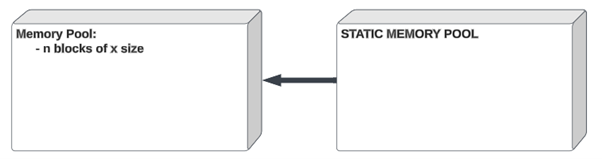
\includegraphics[width=0.9\textwidth]{mem_pool.png}
\end{center}
To implement a memory pool into DocetOS, a static memory pool firstly allocates a predefined block of memory at runtime. Blocks of memory of the required size can then be requested from the static memory pool, which will be aligned to the correct size to prevent fragmentation, and be sent to the memory pool.\hfill\newline
Users can then request a block of memory from the pool and cast it to the desired data type, and then return the memory block to the pool when no longer required. This acts much like malloc() and free() do in a regular system, though as our memory pool defines memory at run time, our implementation is faster.\hfill\newline
Memory blocks are stored within the memory pool as a linked list, having being cast to a struct data type with a pointer to the next block of memory in the list. As modifications to the memory pool required only one store operation in the pool, we protect the memory pool and static memory pool against race conditions using the Cortex-M LDREX and STREX instructions.